\documentclass[12pt]{article}
\usepackage{graphicx} % Required for inserting images
\usepackage{enumitem}
\usepackage{mathtools}
\usepackage{amsmath}
\usepackage{gvv-book}
\usepackage{gvv}

\title{\textbf{4.10.2}}
\author{\textbf{EE25BTECH11004 - Aditya Appana}}
\date{September 14, 2025}

\begin{document}

\maketitle

\section*{Question}
The distance of the point of intersection of the lines $2x$ $-$ $3y + 5= 0$ and $3x + 4y = 0$
from the line $5x$ $-$ $2y = 0$ is \rule{1.5cm}{0.15mm}.

\section*{Solution}

We need to find the point of intersection of the lines $2x$ $-$ $3y + 5= 0$ and $3x + 4y = 0$, which we can do by forming the augmented matrix. \\
\begin{align}
\myvec{2 & -3 & -5 \\ 3 & 4 & 0}
\end{align}

Using row transformations:
\begin{align}
\myvec{2 & -3 & 5 \\ 3 & 4 & 0} \xrightarrow{\text{R_2 \rightarrow $R_2- \frac{3}{2}R_1$}} \myvec{2 & -3 & 5 \\ 0 & \frac{17}{2} & \frac{-15}{2}} 
\end{align} 

Solving, we get the point of intersection as \begin{align}\myvec{\frac{-20}{17} \\ \frac{15}{17}}\end{align}

Two find the distance of this point from the line $5x$ $-$ $2y = 0$, we use the formula:
\begin{align}
\left|\frac{\vec{n}^T\vec{x} - c}{||n||}\right| = d \\
\left|\frac{\myvec{5\\-2}^T\myvec{\frac{-20}{17} \\ \frac{15}{17}}}{\sqrt{5^2 + 2^2}}\right| = 
\left|\frac{-130}{17\sqrt{29}}\right| = \frac{130}{17\sqrt{29}} = d
\end{align}

The distance of the point of intersection of the lines $2x$ $-$ $3y + 5= 0$ and $3x + 4y = 0$
from the line $5x$ $-$ $2y = 0$ is $\frac{130}{17\sqrt{29}}$.


\begin{figure}[H]
    \centering
    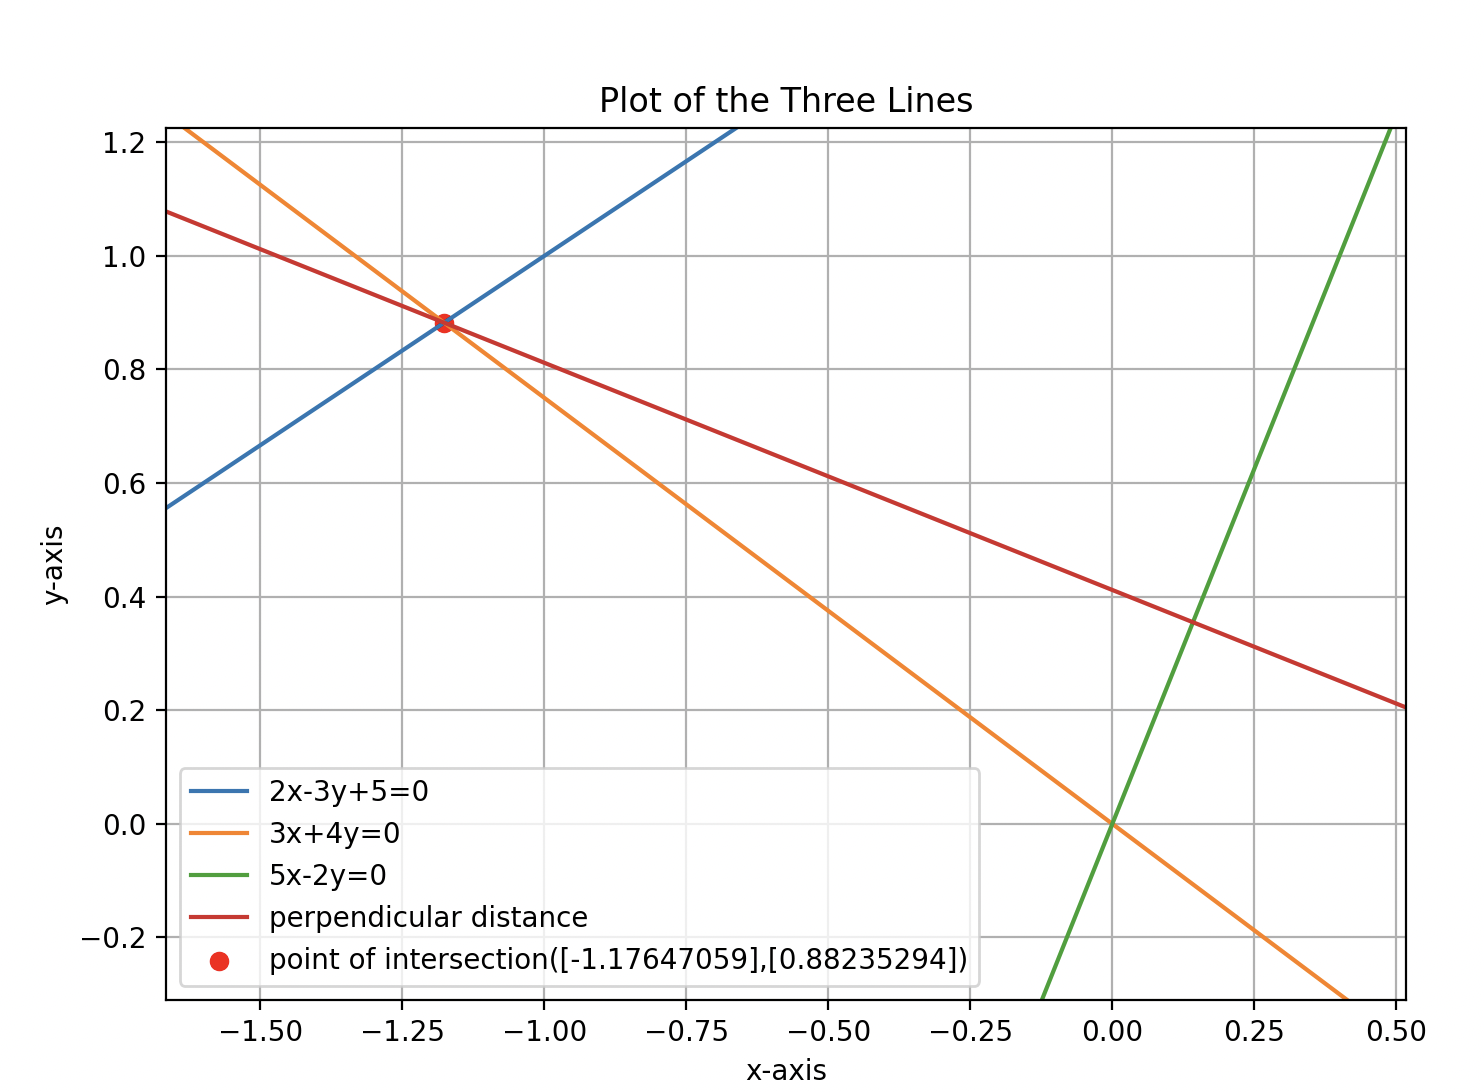
\includegraphics[width=0.9\columnwidth]{Figs/Threelines.png}
    \caption{Plot}
    \label{fig:placeholder}
\end{figure}

\end{document}